\documentclass[11pt]{article}
\usepackage[english]{babel}
% Preambulo comun de los tres documentos (el idioma de babel se carga antes de este archivo)
\usepackage[utf8]{inputenc}
\usepackage[T1]{fontenc}
\usepackage{lmodern}
\usepackage[margin=2.5cm]{geometry}
\usepackage{amsmath,amssymb}
\usepackage{graphicx}
\usepackage{array}
\usepackage{float}
\usepackage{caption}
\usepackage{enumitem}
\usepackage{microtype}
\usepackage[round]{natbib}
\usepackage[hidelinks]{hyperref}
\captionsetup{font=small,labelfont=bf,justification=justified,singlelinecheck=false}
\captionsetup[table]{position=top,skip=6pt}
\renewcommand{\arraystretch}{1.25}
\setlength{\parskip}{0.45em}
\setlength{\parindent}{0pt}
\graphicspath{{figuras/}}
\newcommand{\tabla}[1]{\centering\small\setlength{\tabcolsep}{4.5pt}\input{tablas/#1}}

% Captions of tables and figures (English). Shared by the report and by the standalone PNG renderings.
\newcommand{\capTabA}{Seedling Survival in LHS-1 According to the Proportion of Ionitoponic Substrate. Values Are Expressed as Mean $\pm$ Standard Deviation (SD); $n = 5$ Experimental Units per Group.}
\newcommand{\capTabB}{Analysis of Variance for the Proportion of Ionitoponic Substrate in LHS-1, Partitioned into Two Planned Orthogonal Contrasts.}
\newcommand{\capTabC}{Planned Contrasts for Seedling Survival in LHS-1. Differences Are Expressed in Percentage Points (pp).}
\newcommand{\capTabD}{Sensitivity of the Planned Contrasts to the Choice of Error Term and Unit of Analysis.}
\newcommand{\capTabE}{Contextual Contrasts for Seedling Survival. Differences Are Expressed in Percentage Points (pp).}
\newcommand{\capTabF}{Two-Way Analysis of Variance for Seedling Survival According to Substrate and Treatment.}
\newcommand{\capTabG}{Germination According to Treatment and Substrate. Values Are Expressed as Proportions with Exact (Clopper--Pearson) 95\% Confidence Intervals (CI).}
\newcommand{\capTabH}{Selected Contrasts for Germination, Evaluated at the Seed Level and at the Experimental-Unit Level.}
\newcommand{\capTabI}{Statistical Power of the Pilot Phase and Sample Size Required for a Confirmatory Experiment (Power of 0.80, $\alpha = 0.05$).}
\newcommand{\capFigA}{Seedling survival in LHS-1 according to the proportion of ionitoponic substrate. Points represent group means and bars represent $\pm 1$ standard error (pooled error, 32 degrees of freedom); $n = 5$ experimental units per group.}
\newcommand{\capFigB}{Estimated differences in seedling survival with two-sided 95\% confidence intervals. Dark markers correspond to the planned contrasts of the hypothesis; gray markers correspond to complementary and contextual comparisons.}
\newcommand{\capFigC}{Seedling survival according to treatment and substrate. Points represent group means and bars represent $\pm 1$ standard error (pooled error, 32 degrees of freedom).}
\newcommand{\capFigD}{Germination according to treatment and substrate. Points represent observed proportions and bars represent exact (Clopper--Pearson) 95\% confidence intervals; 20 seeds per group.}
\newcommand{\capFigE}{Statistical power to detect a difference of 20 percentage points in seedling survival as a function of the number of experimental units per group ($\alpha = 0.05$; residual standard deviation of 31.8 percentage points). The horizontal line indicates a power of 0.80.}


\title{\textbf{Statistical Analysis of the Pilot Phase}\\[4pt]
\large Seedling survival and germination of \textit{Raphanus sativus} in the lunar regolith simulant LHS-1 amended with ionitoponic substrate}
\author{}
\date{}

\begin{document}
\maketitle
\vspace{-3em}

\section{Statistical analysis}

\subsection{Experimental design and data}

During the pilot phase, 160 \textit{Raphanus sativus} seeds were evaluated across 40 experimental units using two growth substrates: the lunar regolith simulant LHS-1 and autoclaved river sand. Four nutritional treatments were considered for each substrate: control, conventional nutrient solution, 5\% additive, and 10\% additive. This arrangement corresponds to a $2 \times 4$ factorial design with five experimental units per substrate--treatment combination and four seeds per unit.

The additive treatments correspond to the proportion of ionitoponic substrate incorporated into the growth medium (5\% and 10\%), whereas the control corresponds to the unamended medium (0\%). Germination was expressed as the percentage of sown seeds that germinated in each unit, and survival as the percentage of germinated seeds that survived in each unit. The analysis was carried out from the summary statistics of each substrate--treatment combination (mean $\pm$ standard deviation of the unit-level percentages).

\subsection{Hypothesis and planned contrasts}

We hypothesized that plants grown in the amended simulant would show higher survival than those grown in unamended LHS-1, and that this response would vary with the proportion of ionitoponic substrate in the growth medium. Let $\mu_0$, $\mu_5$, and $\mu_{10}$ denote the mean survival in LHS-1 with 0\%, 5\%, and 10\% of ionitoponic substrate, respectively. The hypothesis was translated into two planned orthogonal contrasts:
\begin{align*}
\text{C1 (effect of the amendment):} \quad & H_0\colon \tfrac{1}{2}(\mu_5 + \mu_{10}) \le \mu_0 & \text{vs.} \quad & H_1\colon \tfrac{1}{2}(\mu_5 + \mu_{10}) > \mu_0,\\[2pt]
\text{C2 (dependence on the proportion):} \quad & H_0\colon \mu_{10} = \mu_5 & \text{vs.} \quad & H_1\colon \mu_{10} \ne \mu_5.
\end{align*}
The component of the hypothesis related to plant development was not evaluated, since no development variables were included in the present analysis.

\subsection{Analysis of seedling survival}

Seedling survival was analyzed by analysis of variance (ANOVA) computed from the group means and standard deviations. The variation among the three proportions of ionitoponic substrate in LHS-1 (2 degrees of freedom) was partitioned into contrasts C1 and C2 (1 degree of freedom each). The error term was the pooled within-group mean square of the eight substrate--treatment combinations (32 degrees of freedom), since all experimental units belonged to the same experiment and were managed under the same procedures.

Because C1 is directional, it was evaluated with a one-sided $t$ test; its two-sided $p$ value is also reported for reference. C2 was evaluated with a two-sided $t$ test. The $p$ values of the two planned contrasts were adjusted with the Holm procedure \citep{holm}. As complementary analyses, each proportion was compared with the unamended control, a set of contextual contrasts was estimated, and the effects of substrate, treatment, and their interaction were examined with a two-way ANOVA, followed by Tukey's test for the comparisons between treatments.

The robustness of the planned contrasts was examined in three ways: (i) estimating the error only from the groups involved in each contrast; (ii) using the Welch--Satterthwaite approximation, which does not assume equal variances \citep{welch,satterthwaite}; and (iii) repeating the comparisons at the seed level with exact tests.

\subsection{Analysis of germination}

Germination was close to 100\% in most groups and three groups showed no variability; therefore, an ANOVA on percentages was not considered appropriate for this variable, and germination was treated as a binomial response. Exact 95\% confidence intervals were calculated for each group \citep{clopper}. Differences between groups were evaluated at the seed level with Fisher's exact test and with Newcombe's confidence interval for the difference between two proportions \citep{newcombe}.

Since the treatments were applied to the experimental units and not to individual seeds, seeds from the same unit cannot be regarded as independent observations \citep{hurlbert}. For this reason, the same comparisons were also evaluated with permutation tests that take the experimental unit as the unit of analysis (10\,000 random rearrangements of the units, stratified by substrate or by treatment as appropriate), and these unit-level results were considered the primary evidence for germination. The number of germinated seeds in each unit was derived from the reported means and standard deviations. The overall effects of treatment and of the substrate--treatment interaction were additionally examined through the analysis of deviance of a binomial model with logit link, with and without a correction for overdispersion.

\subsection{Daily Light Integral (DLI)}

The DLI was recorded daily at each growing location, and each location housed two treatments of the same substrate. Consequently, the DLI was available as four location-level values, and its standard deviation reflects day-to-day variation rather than variation among experimental units. For this reason, the DLI was not included as a covariate in the models; its relationship with survival and germination was explored descriptively through Pearson's correlation among the eight group means.

\subsection{Significance level and software}

A significance level of $\alpha = 0.05$ and 95\% confidence intervals were used throughout. All analyses were performed in R, version 4.3.3 \citep{rcore}.

\section{Results}

\subsection{Seedling survival in LHS-1: test of the hypothesis}

Seedling survival in LHS-1 increased progressively with the proportion of ionitoponic substrate: 55.0\% in the unamended simulant, 65.0\% with 5\%, and 85.0\% with 10\% (Table~\ref{tab:hyp-data}, Figure~\ref{fig:dose}). However, the overall variation among the three proportions was not statistically significant ($F_{2,32} = 1.15$, $p = 0.329$; Table~\ref{tab:anova-dose}).

\begin{table}[H]
\caption{\capTabA}\label{tab:hyp-data}
\tabla{tabA_datos_hipotesis_en}
\end{table}

\begin{figure}[H]
\centering
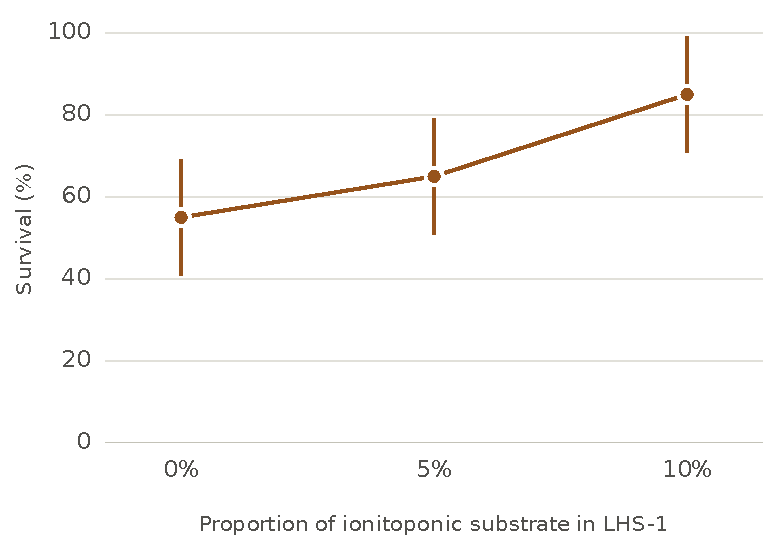
\includegraphics[width=0.72\linewidth]{figA_supervivencia_dosis_en}
\caption{\capFigA}\label{fig:dose}
\end{figure}

\begin{table}[H]
\caption{\capTabB}\label{tab:anova-dose}
\tabla{tabB_anova_dosis_en}
\end{table}

Regarding the first component of the hypothesis (C1), survival in the amended simulant was, on average, 20.0 percentage points higher than in unamended LHS-1 (95\% CI: $-15.5$ to 55.5), a difference that did not reach statistical significance (one-sided $p = 0.130$; two-sided $p = 0.260$). Regarding the second component (C2), survival with 10\% of ionitoponic substrate was 20.0 percentage points higher than with 5\% (95\% CI: $-21.0$ to 61.0; $p = 0.328$). After the Holm adjustment, the $p$ values were 0.260 and 0.328, respectively. Therefore, neither of the two null hypotheses was rejected (Table~\ref{tab:contrasts}, Figure~\ref{fig:forest}).

When each proportion was compared with the unamended control, the difference was 10.0 percentage points for 5\% (one-sided $p = 0.311$) and 30.0 percentage points for 10\% (one-sided $p = 0.073$; Holm-adjusted $p = 0.146$). The latter comparison is equivalent to the linear trend across the three proportions and corresponds to an estimated increase of 3.0 percentage points in survival for each additional 1\% of ionitoponic substrate (95\% CI: $-1.1$ to 7.1).

\begin{table}[H]
\caption{\capTabC}\label{tab:contrasts}
\tabla{tabC_contrastes_en}
\end{table}

\begin{figure}[H]
\centering
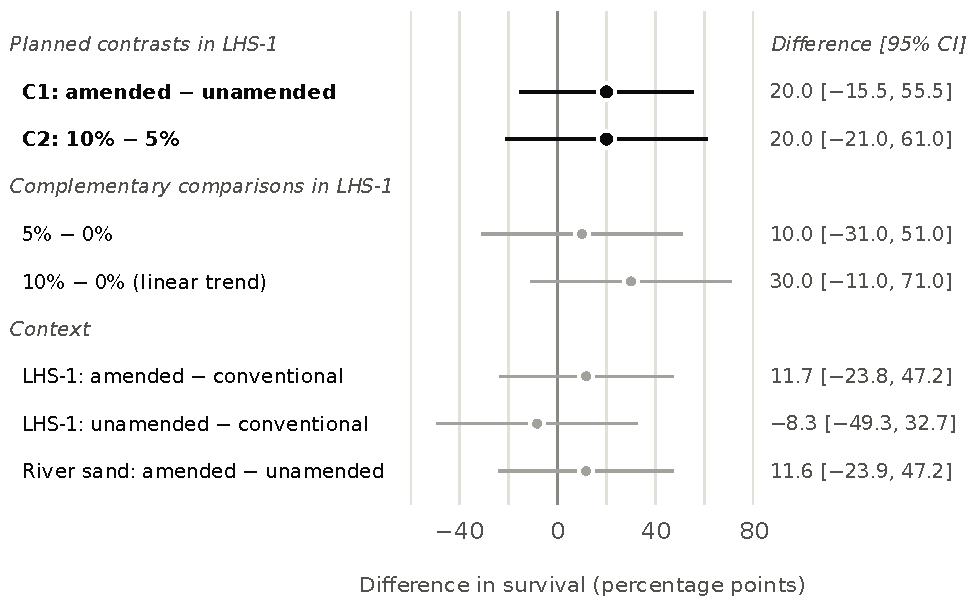
\includegraphics[width=0.95\linewidth]{figB_contrastes_en}
\caption{\capFigB}\label{fig:forest}
\end{figure}

\subsection{Robustness of the result}

The conclusion did not depend on the way in which the experimental error was estimated: the one-sided $p$ value of C1 ranged from 0.112 to 0.136, and the $p$ value of C2 ranged from 0.263 to 0.328 (Table~\ref{tab:sensitivity}). At the seed level, Fisher's exact test led to the same conclusion for C1 (29 of 39 surviving seedlings in the amended simulant vs. 11 of 20 in unamended LHS-1; one-sided $p = 0.113$) and for C2 (16 of 19 vs. 13 of 20; $p = 0.273$).

The exact test for trend across the three proportions at the seed level yielded a one-sided $p$ value of 0.038. Nevertheless, this analysis assumes that the seeds of the same experimental unit respond independently, and the variability observed among units was approximately 1.6 times larger than expected under that assumption. When this overdispersion was taken into account, the $p$ value was 0.059, in agreement with the unit-level analysis ($p = 0.073$). Consequently, the increasing trend should be regarded as suggestive rather than conclusive.

\begin{table}[H]
\caption{\capTabD}\label{tab:sensitivity}
\tabla{tabD_sensibilidad_en}
\end{table}

\subsection{Context of the hypothesis}

Survival in unamended LHS-1 did not differ significantly from that observed in LHS-1 with conventional nutrient solution ($-8.3$ percentage points; $p = 0.683$) or in unamended river sand ($+10.0$ percentage points; $p = 0.623$). Likewise, the amended simulant did not differ significantly from LHS-1 with conventional nutrient solution ($+11.7$ percentage points; 95\% CI: $-23.8$ to 47.2; $p = 0.507$). In river sand, the amendment was associated with a difference of similar magnitude ($+11.6$ percentage points; $p = 0.509$), and the effect of the amendment did not differ between substrates ($p = 0.737$; Table~\ref{tab:context}).

\begin{table}[H]
\caption{\capTabE}\label{tab:context}
\tabla{tabE_contexto_en}
\end{table}

\subsection{Seedling survival according to substrate and treatment}

Considering the complete factorial design, mean survival was 67.1\% in LHS-1 and 51.7\% in river sand, a difference of 15.4 percentage points (95\% CI: $-5.1$ to 35.9) that was not statistically significant ($F_{1,32} = 2.35$, $p = 0.135$). Neither the effect of treatment ($F_{3,32} = 0.83$, $p = 0.489$) nor the substrate--treatment interaction ($F_{3,32} = 0.15$, $p = 0.927$) was significant (Table~\ref{tab:anova-factorial}, Figure~\ref{fig:factorial}), and none of the pairwise comparisons between treatments reached significance (Tukey's test, $p \ge 0.438$).

\begin{table}[H]
\caption{\capTabF}\label{tab:anova-factorial}
\tabla{tabF_anova_factorial_en}
\end{table}

\begin{figure}[H]
\centering
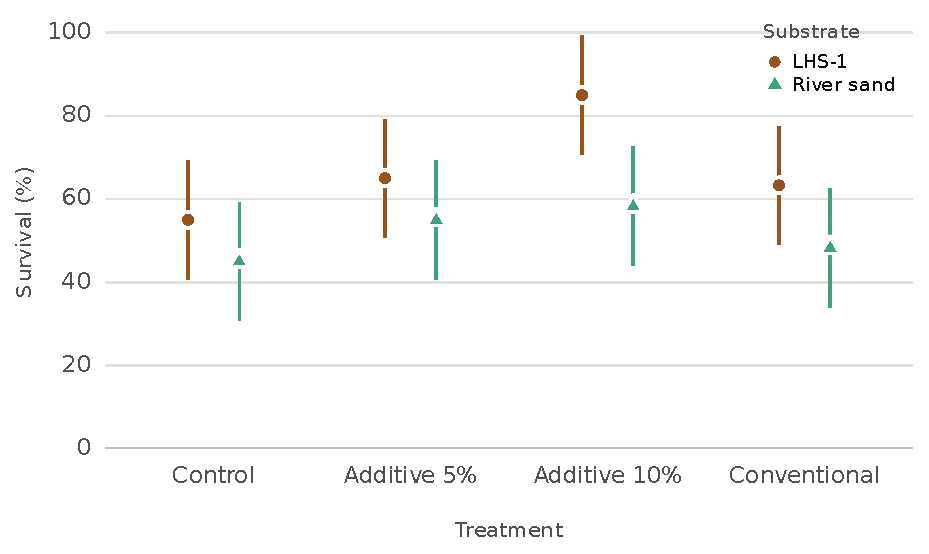
\includegraphics[width=0.85\linewidth]{figC_supervivencia_factorial_en}
\caption{\capFigC}\label{fig:factorial}
\end{figure}

\subsection{Germination}

Overall germination was identical in both substrates (72 of 80 seeds, 90.0\%; difference of 0.0 percentage points, 95\% CI: $-9.8$ to 9.8). The lowest values were observed in LHS-1 with conventional nutrient solution (13 of 20 seeds, 65.0\%) and in river sand with 5\% additive (15 of 20 seeds, 75.0\%; Table~\ref{tab:germination}, Figure~\ref{fig:germination}).

\begin{table}[H]
\caption{\capTabG}\label{tab:germination}
\tabla{tabG_germinacion_en}
\end{table}

\begin{figure}[H]
\centering
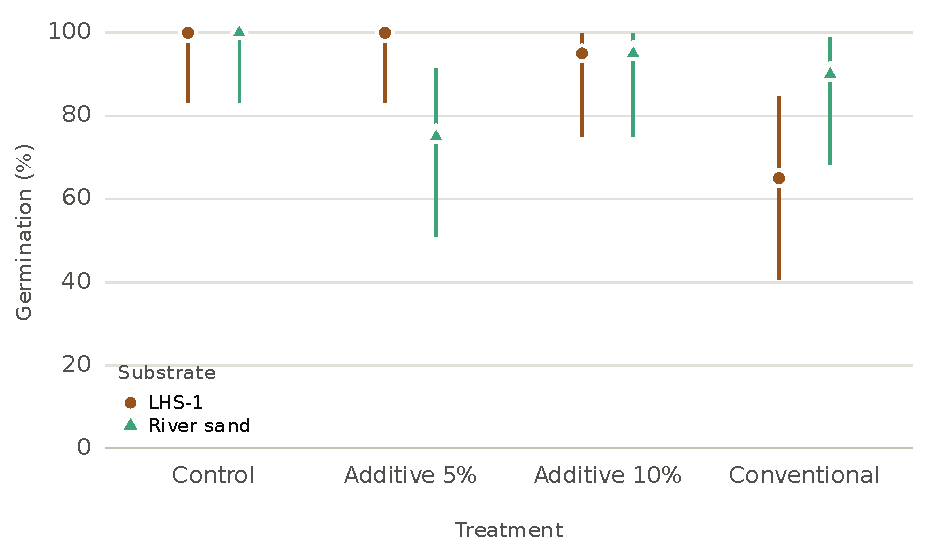
\includegraphics[width=0.85\linewidth]{figD_germinacion_en}
\caption{\capFigD}\label{fig:germination}
\end{figure}

At the seed level, germination differed among treatments (Fisher's exact test, $p = 0.003$), mainly because of the lower germination observed with the conventional nutrient solution (31 of 40 seeds vs. 40 of 40 in the control; Holm-adjusted $p = 0.007$). However, when the experimental unit was taken as the unit of analysis, none of the comparisons reached statistical significance (Table~\ref{tab:germ-contrasts}). This difference between the two levels of analysis is explained by the fact that the non-germinated seeds in LHS-1 with conventional nutrient solution were concentrated in three of the five experimental units, one of which showed no germination. In agreement with this, when overdispersion was taken into account in the binomial model, the evidence was weaker for the treatment effect ($p$ between 0.035 and 0.046) and for the substrate--treatment interaction ($p$ between 0.082 and 0.101). Therefore, the lower germination associated with the conventional nutrient solution in LHS-1 should be considered a preliminary observation.

\begin{table}[H]
\caption{\capTabH}\label{tab:germ-contrasts}
\tabla{tabH_contrastes_germinacion_en}
\end{table}

\subsection{Daily Light Integral (DLI)}

No association was observed between the DLI and seedling survival among the eight group means ($r = -0.02$; 95\% CI: $-0.71$ to 0.69; $p = 0.964$), nor between the DLI and germination ($r = 0.42$; 95\% CI: $-0.40$ to 0.87; $p = 0.295$). Because each growing location housed specific treatments, the effect of light cannot be separated from the effect of the treatments, and these results are only descriptive.

\section{Interpretation}

The results of the pilot phase are directionally consistent with the hypothesis: seedling survival in LHS-1 increased progressively as the proportion of ionitoponic substrate increased (55.0\%, 65.0\%, and 85.0\%). Nevertheless, with five experimental units per group, the observed differences did not reach statistical significance, and the confidence intervals were wide: they are compatible both with the absence of an effect and with a considerable improvement in survival. Consequently, the pilot phase does not allow the hypothesis to be confirmed or ruled out; the result should be understood as inconclusive rather than as evidence that the amendment has no effect.

With the available survival data, the premise of a low nutrient availability in LHS-1 could not be verified, since survival in the unamended simulant was not lower than that observed with the conventional nutrient solution or in river sand. It is possible that variables related to plant development are more informative than survival for this purpose; this aspect remains to be evaluated. In the same way, the available data do not allow us to state that the amendment performs equally to the conventional nutrient solution, because the absence of a significant difference is not equivalent to a demonstration of equivalence.

Regarding the substrates, germination was the same in LHS-1 and in river sand, and survival in LHS-1 was not lower than in river sand; the confidence interval of the difference ($-5.1$ to 35.9 percentage points) suggests that a marked reduction in survival attributable to the simulant is unlikely under the conditions evaluated.

\section{Limitations}

The following aspects should be considered when interpreting these results:

\begin{itemize}[leftmargin=1.4em,itemsep=2pt]
\item \textbf{Sample size.} With five experimental units per group, the statistical power to detect the observed differences was low (0.30 for C1 and 0.16 for C2; Table~\ref{tab:power}).
\item \textbf{Number of seeds per unit.} With four seeds per unit, the percentages of each unit can only take a few values, which limits the precision of the estimates.
\item \textbf{Summary-level data.} The analysis was based on means and standard deviations; therefore, the distribution of the unit-level values could not be examined. In addition, some of the reported dispersion values could not be reproduced exactly from the design described, so it would be advisable to verify them against the unit-level records. This aspect did not affect the conclusions: when the closest reproducible values were used, the error mean square changed by 2.6\% and no decision was modified.
\item \textbf{Light environment.} In LHS-1, the group with 10\% of ionitoponic substrate was located at a growing location with a lower DLI (9.52 mol$\cdot$m$^{-2}\cdot$day$^{-1}$) than the control and 5\% groups (10.73 mol$\cdot$m$^{-2}\cdot$day$^{-1}$). Consequently, the comparisons that involve the 10\% group are partially confounded with the growing location. Only the comparisons between 5\% and the control, and between 10\% and the conventional nutrient solution, were made within the same location.
\item \textbf{Exploratory comparisons.} Apart from the two planned contrasts, the remaining comparisons are exploratory and were not adjusted jointly for multiplicity; they should be interpreted as a guide for future experiments.
\end{itemize}

\section{Recommendations}

Based on the above, we suggest considering the following points for the confirmatory phase:

\begin{enumerate}[leftmargin=1.6em,itemsep=2pt]
\item \textbf{Increase the number of experimental units.} Under the variability observed in the pilot phase, approximately 24 experimental units per group would be required to detect a difference of 20 percentage points between the amended and unamended simulant with a power of 0.80, and approximately 41 units per group to detect the same difference between the two proportions (Table~\ref{tab:power}, Figure~\ref{fig:power}). It would be preferable to define beforehand the smallest difference considered relevant and to calculate the sample size from that value.
\item \textbf{Increase the number of seeds per unit}, so that the percentage of each unit is estimated with greater precision.
\item \textbf{Randomize the position of the units} among the growing locations, or arrange all treatments within each location as blocks, and, if possible, record the DLI for each unit. This would allow the effect of light to be separated from the effect of the treatments.
\item \textbf{Record and analyze the counts of each unit} (seeds sown, germinated, and surviving). With these data, germination and survival could be analyzed with a binomial mixed model that includes the experimental unit as a random effect, which is the most appropriate approach for this type of response.
\item \textbf{Include variables of plant development}, so that the component of the hypothesis related to development can be evaluated.
\item \textbf{Define the analysis before the experiment}: the primary response variable, the planned contrasts, and the significance level.
\item \textbf{If the objective is to show that the amendment performs comparably to the conventional nutrient solution}, define beforehand the margin of difference considered acceptable and apply an equivalence or non-inferiority test.
\item \textbf{Consider additional proportions of ionitoponic substrate}, which would allow the shape of the response to be described with greater detail.
\end{enumerate}

\begin{table}[H]
\caption{\capTabI}\label{tab:power}
\tabla{tabI_potencia_en}
\end{table}

\begin{figure}[H]
\centering
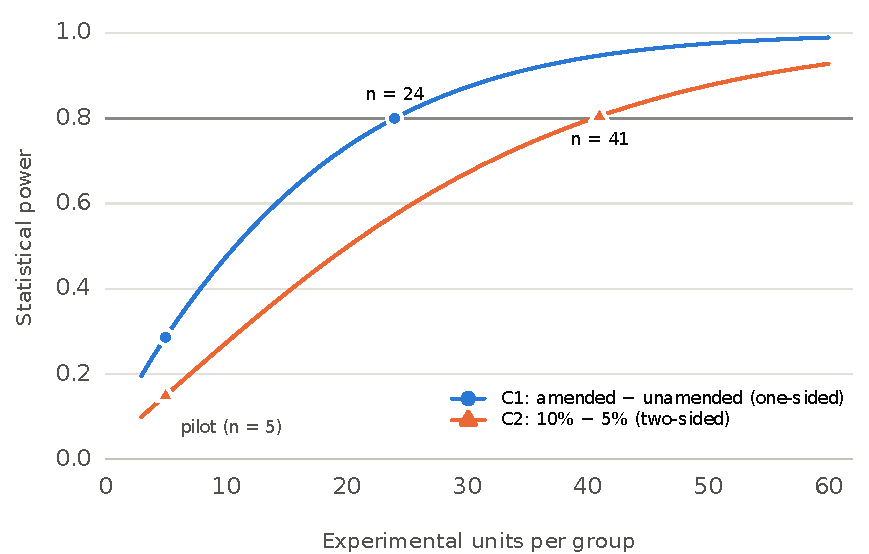
\includegraphics[width=0.8\linewidth]{figE_potencia_en}
\caption{\capFigE}\label{fig:power}
\end{figure}

\begin{thebibliography}{9}
\bibitem[Clopper and Pearson(1934)]{clopper} Clopper, C. J., \& Pearson, E. S. (1934). The use of confidence or fiducial limits illustrated in the case of the binomial. \textit{Biometrika}, 26(4), 404--413.
\bibitem[Holm(1979)]{holm} Holm, S. (1979). A simple sequentially rejective multiple test procedure. \textit{Scandinavian Journal of Statistics}, 6(2), 65--70.
\bibitem[Hurlbert(1984)]{hurlbert} Hurlbert, S. H. (1984). Pseudoreplication and the design of ecological field experiments. \textit{Ecological Monographs}, 54(2), 187--211.
\bibitem[Newcombe(1998)]{newcombe} Newcombe, R. G. (1998). Interval estimation for the difference between independent proportions: comparison of eleven methods. \textit{Statistics in Medicine}, 17(8), 873--890.
\bibitem[R Core Team(2024)]{rcore} R Core Team (2024). \textit{R: A language and environment for statistical computing}. R Foundation for Statistical Computing, Vienna, Austria.
\bibitem[Satterthwaite(1946)]{satterthwaite} Satterthwaite, F. E. (1946). An approximate distribution of estimates of variance components. \textit{Biometrics Bulletin}, 2(6), 110--114.
\bibitem[Welch(1947)]{welch} Welch, B. L. (1947). The generalization of ``Student's'' problem when several different population variances are involved. \textit{Biometrika}, 34(1--2), 28--35.
\end{thebibliography}

\end{document}
